% Provenance (never printed): cycle 3 "La planete Terre" (the shaping of
% landscapes: erosion, transport and deposition by running water; rivers
% from source to mouth; floods); see sources/book1/PROVENANCE.md.
% Book 1, grade 5, chapter 1.
\chapter{Water vormt het land}\label{ch:g5:water-shapes-the-land}

De hele nacht trommelde de storm op het dak van de school. 's Ochtends
klaart de lucht op, en Lena en Tom rennen naar het beekje achter het
schoolplein. Gisteren was het helder en rustig: ze konden de \omterm{def:g3:stones-pebbles-sand:pebble}{kiezels} op
de bodem tellen. Vandaag is het breed, snel en bruin, de kleur van
chocolademelk. Het voert takjes en bladeren mee, en iets wat ze niet
één voor één kunnen zien: \omterm{def:g3:stones-pebbles-sand:sand}{slib} en \omterm{def:g3:stones-pebbles-sand:sand}{zand}, losgescheurd uit de oevers en uit
de akkers stroomopwaarts.

``Waar gaat al dat \omterm{def:g3:stones-pebbles-sand:sand}{slib} naartoe?'' vraagt Tom. Stroomafwaarts, elke minuut
een stukje verder. De beek voert het land weg, korrel voor korrel. In dit
hoofdstuk volgen we die korrels, van het \omterm{def:g3:stones-pebbles-sand:rock}{gesteente} waar ze vandaan komen
tot de plek waar ze tot rust komen.

\begin{omfigure}
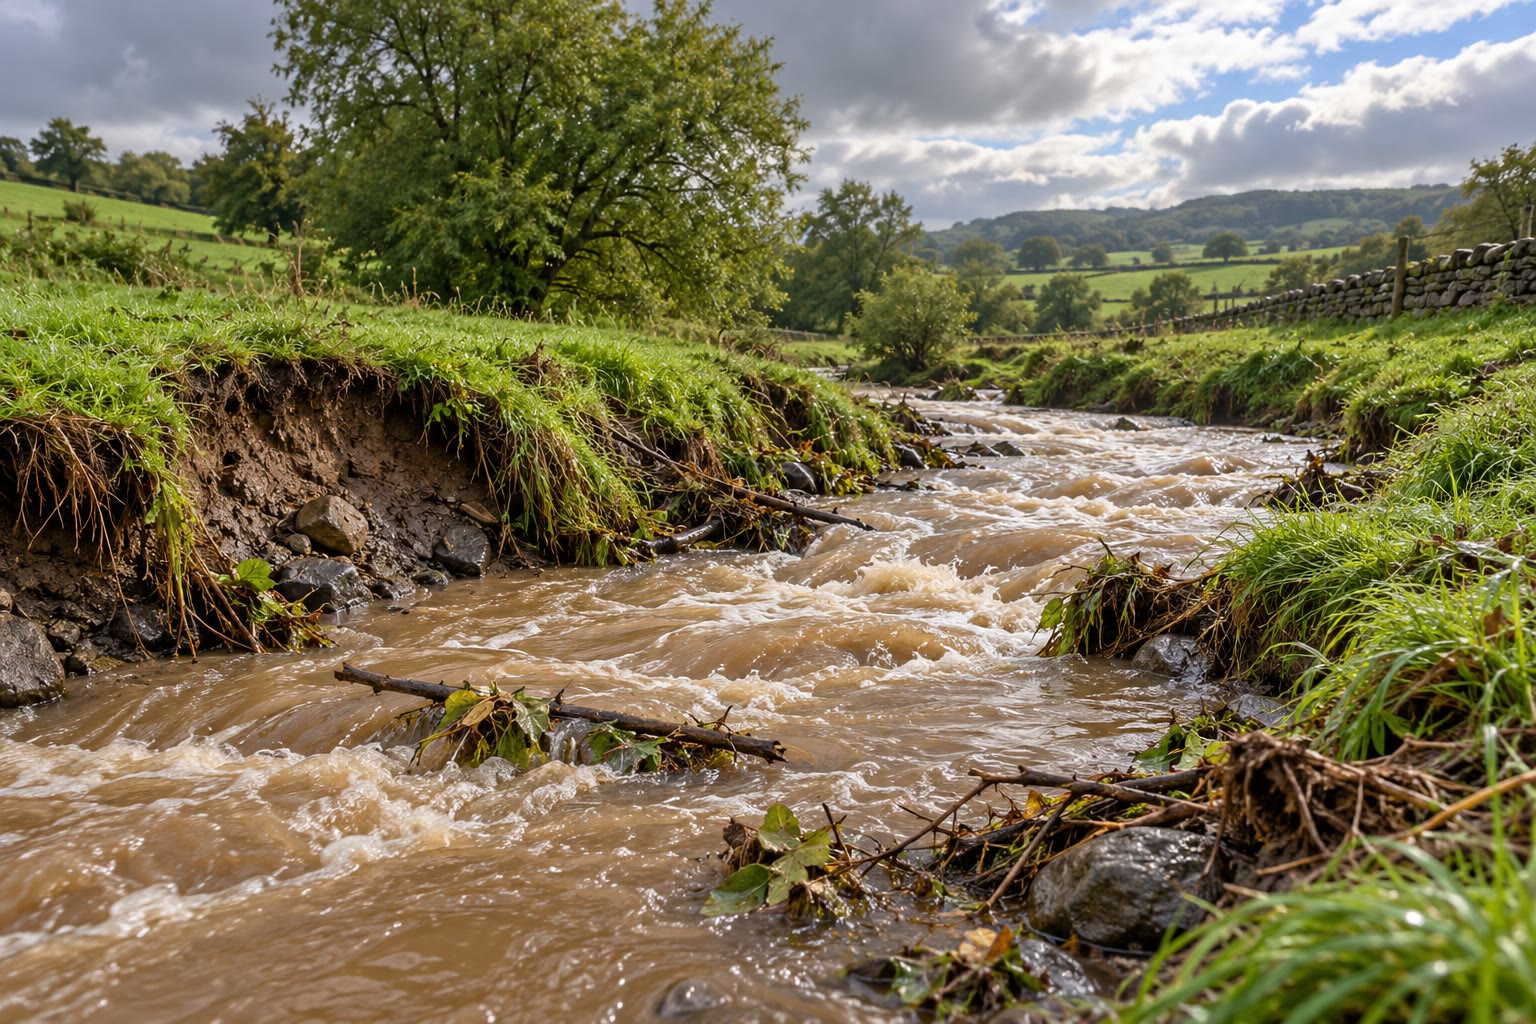
\includegraphics[width=0.5\linewidth]{images/book1/ai/g5-brown-stream.jpg}

{\small Een beek de ochtend na een storm: het water is bruin van het \omterm{def:g3:stones-pebbles-sand:sand}{slib}
en het \omterm{def:g3:stones-pebbles-sand:sand}{zand} dat het meevoert.}
\end{omfigure}

\begin{recall}
\omterm{def:g3:stones-pebbles-sand:rock}{Gesteente} is het harde materiaal van de Aarde; in stukken gebroken geeft
het stenen, \omterm{def:g3:stones-pebbles-sand:pebble}{kiezels} die door het water rond zijn geslepen, \omterm{def:g3:stones-pebbles-sand:sand}{zand} waarvan we
de korrels één voor één kunnen zien, en \omterm{def:g3:stones-pebbles-sand:sand}{slib} waarvan de korrels te klein
zijn om te zien (\cref{ch:g3:stones-pebbles-sand}). Een \omterm{def:g1:landscapes-around-us:water}{rivier} stroomt de
hele tijd door een lange bedding, van hoger land naar beneden, naar een
\omterm{def:g1:landscapes-around-us:water}{meer} of naar de \omterm{def:g2:water-on-earth:ocean}{zee} (\cref{ch:g1:landscapes-around-us}). \omterm{def:g4:clouds-rain-snow:precipitation}{Regen} die op het
land valt, stroomt weg naar beken en \omterm{def:g1:landscapes-around-us:water}{rivieren}, die het water terugbrengen
naar de \omterm{def:g2:water-on-earth:ocean}{zee} (\cref{ch:g2:water-on-earth}).
\end{recall}

\section{Gesteente breekt waar het ligt}

Zelfs het hardste \omterm{def:g3:stones-pebbles-sand:rock}{gesteente} blijft niet eeuwig bestaan. Waar het in de open
lucht ligt, onder zon, \omterm{def:g4:clouds-rain-snow:precipitation}{regen} en vorst, barst en brokkelt het langzaam af.

\begin{definition}[Verwering]\label{def:g5:water-shapes-the-land:weathering}
\emph{Verwering}\index{verwering} is het langzame uiteenvallen van \omterm{def:g3:stones-pebbles-sand:rock}{gesteente}
op de plek waar het ligt, door vorst, door water, door de wortels van
planten en door warmte en kou. Het \omterm{def:g3:stones-pebbles-sand:rock}{gesteente} valt in stukken uiteen, maar
de stukken blijven liggen waar ze zijn.
\end{definition}

Vorst is een van de sterkste werktuigen van de \omterm{def:g5:water-shapes-the-land:weathering}{verwering}. Regenwater
sijpelt in een smalle spleet in het \omterm{def:g3:stones-pebbles-sand:rock}{gesteente}. In een koude nacht bevriest
het, en water dat bevriest neemt iets meer ruimte in: het ijs duwt tegen de
wanden van de spleet en maakt die een heel klein beetje wijder. De volgende
dag smelt het ijs, er sijpelt meer water in, en de nacht daarna bevriest
het opnieuw. Na veel winters breekt er een stuk \omterm{def:g3:stones-pebbles-sand:rock}{gesteente} af.

\begin{omfigure}
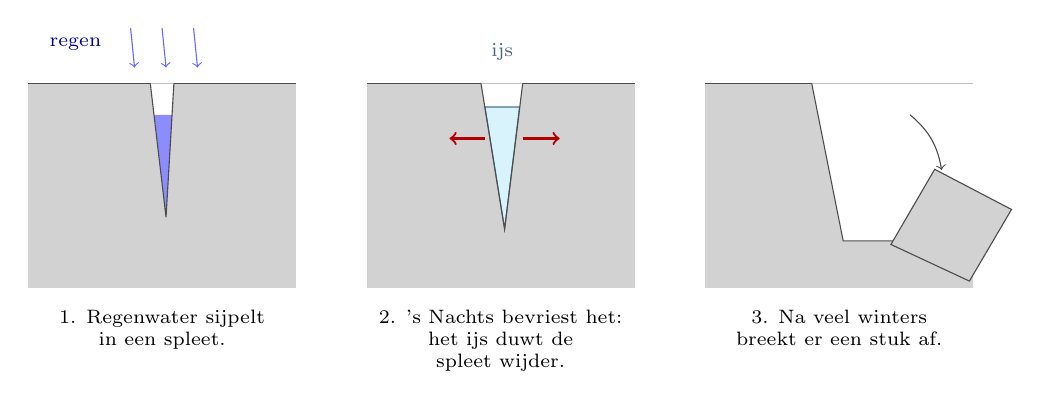
\begin{tikzpicture}[x=1cm, y=1cm, font=\scriptsize]
  \foreach \i/\t in {0/{1. Regenwater sijpelt\\in een spleet.},
                     4.3/{2. 's Nachts bevriest het:\\het ijs duwt de\\spleet wijder.},
                     8.6/{3. Na veel winters\\breekt er een stuk af.}} {
    \begin{scope}[xshift=\i cm]
      \fill[gray!35] (0,0) rectangle (3.4,2.6);
      \draw[gray!60!black] (0,2.6) -- (3.4,2.6);
      \node[align=center, anchor=north] at (1.7,-0.15) {\t};
    \end{scope}
  }
  % panel 1: thin crack with water
  \fill[white] (1.55,2.6) -- (1.75,0.9) -- (1.85,2.6) -- cycle;
  \fill[blue!45] (1.6,2.2) -- (1.75,0.9) -- (1.83,2.2) -- cycle;
  \draw[gray!60!black] (1.55,2.6) -- (1.75,0.9) -- (1.85,2.6);
  \foreach \x in {1.3,1.7,2.1} \draw[blue!60, ->] (\x,3.3) -- (\x+0.05,2.8);
  \node[blue!60!black] at (0.6,3.1) {regen};
  % panel 2: wider crack with ice
  \begin{scope}[xshift=4.3cm]
    \fill[white] (1.45,2.6) -- (1.75,0.75) -- (1.98,2.6) -- cycle;
    \fill[cyan!15] (1.5,2.3) -- (1.75,0.75) -- (1.94,2.3) -- cycle;
    \draw[cyan!50!black] (1.5,2.3) -- (1.75,0.75) -- (1.94,2.3) -- cycle;
    \draw[gray!60!black] (1.45,2.6) -- (1.75,0.75) -- (1.98,2.6);
    \draw[red!70!black, thick, <-] (1.05,1.9) -- (1.5,1.9);
    \draw[red!70!black, thick, ->] (1.98,1.9) -- (2.45,1.9);
    \node[cyan!40!black] at (1.72,3.0) {ijs};
  \end{scope}
  % panel 3: broken block
  \begin{scope}[xshift=8.6cm]
    \fill[white] (1.35,2.6) -- (1.75,0.6) -- (3.4,0.6) -- (3.4,2.6) -- cycle;
    \draw[gray!60!black] (1.35,2.6) -- (1.75,0.6) -- (3.4,0.6);
    \fill[gray!35, draw=gray!60!black, rotate around={-25:(2.9,0.3)}]
      (2.3,0.3) -- (2.4,1.4) -- (3.5,1.35) -- (3.4,0.3) -- cycle;
    \draw[gray!60!black, ->] (2.6,2.2) to[bend left=20] (3.0,1.5);
  \end{scope}
\end{tikzpicture}

{\small Vorst breekt \omterm{def:g3:stones-pebbles-sand:rock}{gesteente}. Elke vorstnacht duwt het ijs in een spleet
een klein beetje; na veel winters is de spleet wijd genoeg om een stuk te
laten afbreken.}
\end{omfigure}

Onder een kale rotswand hoog in de \omterm{def:g1:landscapes-around-us:landform}{bergen} glijden en tuimelen de stukken
die door de vorst zijn afgebroken naar beneden, en ze stapelen zich op tot
een helling van scherpe stenen. Ze zijn niet rond: er heeft nog geen water
mee gerold.

\begin{omfigure}
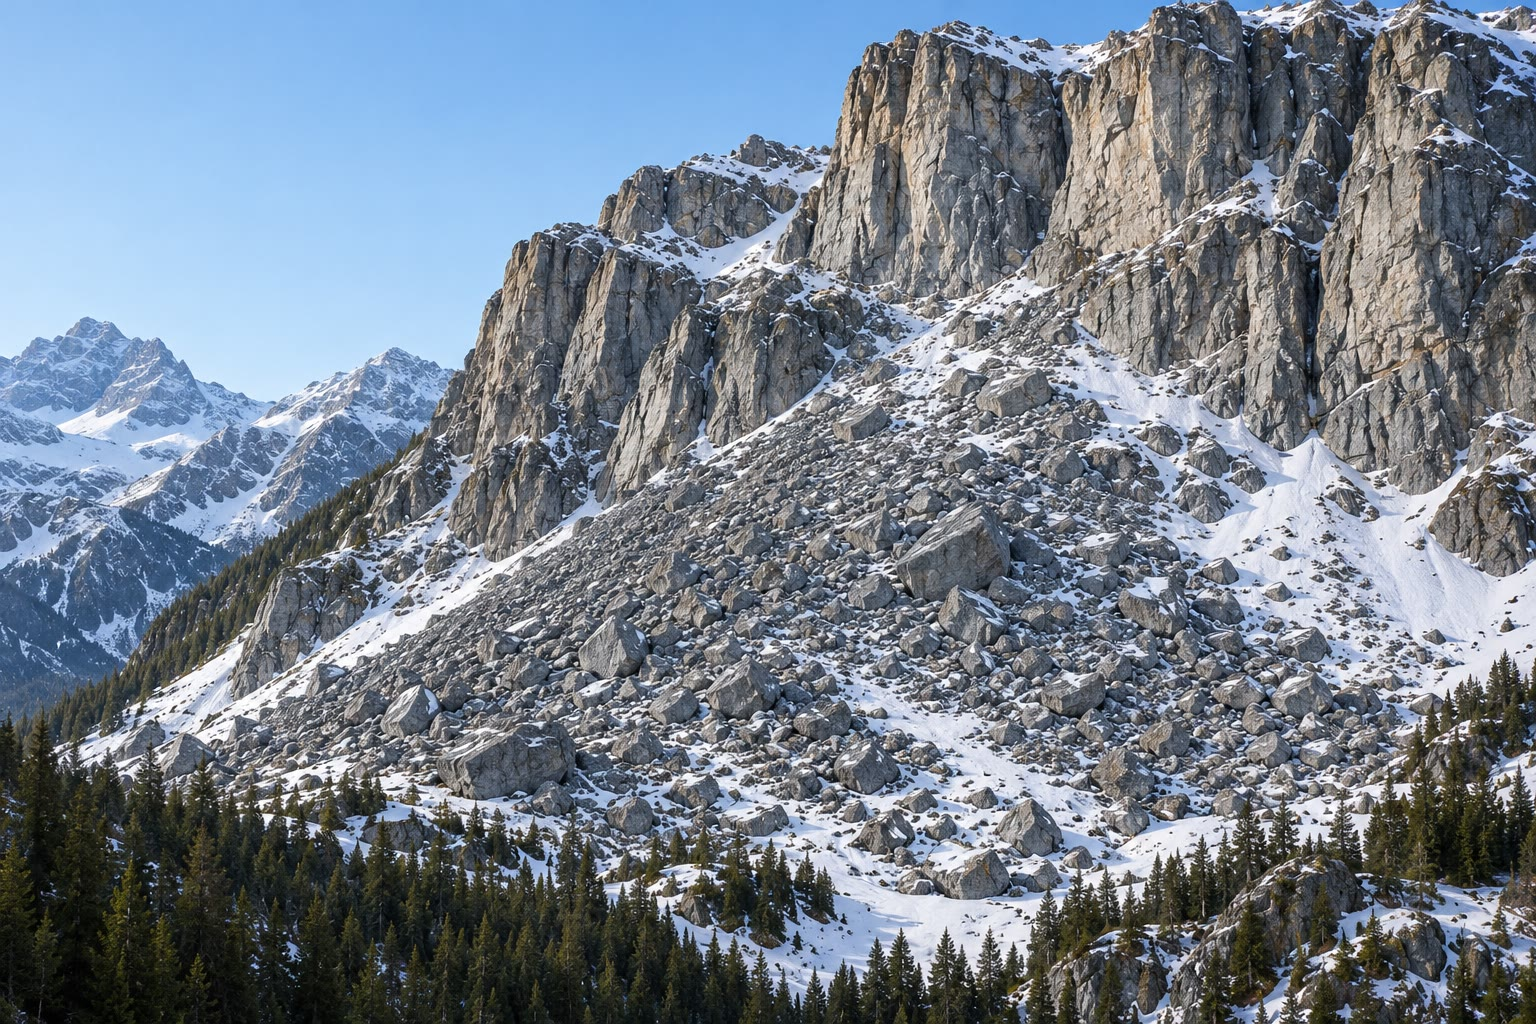
\includegraphics[width=0.5\linewidth]{images/book1/ai/g5-frost-scree.jpg}

{\small Onder een rotswand in de \omterm{def:g1:landscapes-around-us:landform}{bergen} een helling van scherpe stenen die
door de vorst zijn afgebroken, gezien vanaf de overkant van het \omterm{def:g1:landscapes-around-us:landform}{dal}.}
\end{omfigure}

Ook planten helpen mee. Een boomwortel kruipt in een spleet en splijt het
\omterm{def:g3:stones-pebbles-sand:rock}{gesteente} als een langzame wig, terwijl hij jaar na jaar dikker wordt.
Regenwater zelf maakt sommige \omterm{def:g3:stones-pebbles-sand:rock}{gesteenten} langzaam zacht en verandert ze in
klei en \omterm{def:g3:stones-pebbles-sand:sand}{zand}: zo krijgt de bodem zijn minerale korrels.

\section{Water voert de stukken weg}

Als het \omterm{def:g3:stones-pebbles-sand:rock}{gesteente} eenmaal gebroken is, kunnen de stukken bewegen. Iets
moet ze meenemen.

\begin{definition}[Erosie]\label{def:g5:water-shapes-the-land:erosion}
\emph{Erosie}\index{erosie} is het afslijten van het land en het wegvoeren
van de stukken \omterm{def:g3:stones-pebbles-sand:rock}{gesteente}, vooral door stromend water, maar ook door de
wind, door ijs en door de golven van de \omterm{def:g2:water-on-earth:ocean}{zee}.
\end{definition}

Stromend water doet het meeste werk. De \omterm{def:g4:clouds-rain-snow:precipitation}{regen} spoelt grond en korrels de
hellingen af naar de beken; de beken scheuren meer los uit hun eigen
oevers, zoals de beek van Tom en Lena na de storm. Hoe sneller het water
stroomt, hoe meer het kan meevoeren en hoe groter de stukken die het kan
verplaatsen: een kalme beek voert alleen fijn \omterm{def:g3:stones-pebbles-sand:sand}{slib} mee; een beek die
buiten haar oevers treedt, rolt \omterm{def:g3:stones-pebbles-sand:pebble}{kiezels} en zelfs rotsblokken over haar
bodem.

Onderweg botsen de stenen tegen elkaar en tegen de bodem. Hun hoeken
breken af en ze worden ronde \omterm{def:g3:stones-pebbles-sand:pebble}{kiezels}, daarna steeds kleinere korrels: \omterm{def:g3:stones-pebbles-sand:sand}{zand}
en \omterm{def:g3:stones-pebbles-sand:sand}{slib}.

De wind doet hetzelfde werk op droge plaatsen, waar niets het \omterm{def:g3:stones-pebbles-sand:sand}{zand}
vasthoudt: hij blaast het op tot duinen. IJs, in de \omterm{def:g1:landscapes-around-us:landform}{bergen} en bij de \omterm{def:g3:continents-and-oceans:poles}{polen},
sleept onder zijn grote gewicht stenen mee. Aan de \omterm{def:g1:landscapes-around-us:water}{kust} beuken de golven
tegen de kliffen en rollen ze de \omterm{def:g3:stones-pebbles-sand:pebble}{kiezels} van het strand heen en weer.

\begin{remark}[Hoeveel?]\label{rem:g5:water-shapes-the-land:how-much}
Samen brengen alle \omterm{def:g1:landscapes-around-us:water}{rivieren} van de wereld elk jaar meer dan 12 miljard ton
\omterm{def:g3:stones-pebbles-sand:sand}{slib} en \omterm{def:g3:stones-pebbles-sand:sand}{zand} naar de \omterm{def:g2:water-on-earth:ocean}{zee}. Dat is ongeveer een miljard ton per maand.
% ledger: syvitski:modern-flux
\end{remark}

\section{Water legt de stukken neer}

Een \omterm{def:g1:landscapes-around-us:water}{rivier} kan haar lading niet eeuwig meedragen. Waar ze langzamer gaat
stromen, heeft ze niet meer de kracht om haar grootste korrels te
verplaatsen, en die zakken naar de bodem.

\begin{definition}[Afzetting]\label{def:g5:water-shapes-the-land:deposition}
\emph{Afzetting}\index{afzetting} is het neerleggen van de stukken
\omterm{def:g3:stones-pebbles-sand:rock}{gesteente} die door water, wind of ijs zijn meegevoerd, waar die langzamer
gaan en tot stilstand komen.
\end{definition}

De zwaarste stukken zakken het eerst: \omterm{def:g3:stones-pebbles-sand:pebble}{kiezels} vallen waar de stroming een
beetje afneemt, \omterm{def:g3:stones-pebbles-sand:sand}{zand} waar ze nog meer vertraagt, en het fijne \omterm{def:g3:stones-pebbles-sand:sand}{slib} pas waar
het water bijna stilstaat, in een \omterm{def:g1:landscapes-around-us:water}{meer} of in de \omterm{def:g2:water-on-earth:ocean}{zee}. Daarom is de bodem
van een \omterm{def:g1:landscapes-around-us:water}{rivier} in de \omterm{def:g1:landscapes-around-us:landform}{bergen} bezaaid met \omterm{def:g3:stones-pebbles-sand:pebble}{kiezels}, en dicht bij de \omterm{def:g2:water-on-earth:ocean}{zee}
zanderig of slibberig.

\omterm{def:g5:water-shapes-the-land:weathering}{Verwering}, \omterm{def:g5:water-shapes-the-land:erosion}{erosie} en \omterm{def:g5:water-shapes-the-land:deposition}{afzetting} zijn drie stappen van één lange reis: het
\omterm{def:g3:stones-pebbles-sand:rock}{gesteente} breekt waar het ligt, de stukken worden weggevoerd en ze worden
ergens anders neergelegd. Langzaam verplaatst water de \omterm{def:g1:landscapes-around-us:landform}{bergen}, korrel voor
korrel, naar de \omterm{def:g1:landscapes-around-us:landform}{vlakten} en de \omterm{def:g2:water-on-earth:ocean}{zee}.

\begin{method}[Benoemen wat water doet]\label{met:g5:water-shapes-the-land:naming}
Om te benoemen wat er met \omterm{def:g3:stones-pebbles-sand:rock}{gesteente} gebeurt in een plaatje of een verhaal,
stel je drie vragen:
\begin{enumerate}
  \item Breekt het \omterm{def:g3:stones-pebbles-sand:rock}{gesteente}, maar blijven de stukken waar ze zijn?
        Dat is \emph{\omterm{def:g5:water-shapes-the-land:weathering}{verwering}}.
  \item Slijten de stukken af en worden ze weggevoerd? Dat is
        \emph{\omterm{def:g5:water-shapes-the-land:erosion}{erosie}}.
  \item Komen de stukken tot rust en stapelen ze zich op? Dat is
        \emph{\omterm{def:g5:water-shapes-the-land:deposition}{afzetting}}.
\end{enumerate}
\end{method}

\begin{example}[De beek na de storm]\label{ex:g5:water-shapes-the-land:stream}
Het bruine water van de beek van Tom en Lena voert \omterm{def:g3:stones-pebbles-sand:sand}{slib} mee dat uit de
oevers is gescheurd: dat is \omterm{def:g5:water-shapes-the-land:erosion}{erosie}. Een week later is de beek weer helder,
en een dun laagje \omterm{def:g3:stones-pebbles-sand:sand}{slib} bedekt de bodem van de rustige poel aan het eind
van het schoolplein: dat is \omterm{def:g5:water-shapes-the-land:deposition}{afzetting}.
\end{example}

\section{Een rivier van bron tot monding}

Elke \omterm{def:g1:landscapes-around-us:water}{rivier} heeft een begin en een einde.

\begin{definition}[Bron, monding en zijrivier]\label{def:g5:water-shapes-the-land:source-mouth}
De \emph{bron}\index{bron (van een rivier)} van een \omterm{def:g1:landscapes-around-us:water}{rivier} is de plek waar
ze begint: een bron in de grond, een smeltende gletsjer, of een hoog, nat
gebied waar veel piepkleine beekjes ontspringen. Haar
\emph{monding}\index{monding (van een rivier)} is de plek waar ze eindigt,
waar ze uitstroomt in de \omterm{def:g2:water-on-earth:ocean}{zee}, een \omterm{def:g1:landscapes-around-us:water}{meer} of een grotere \omterm{def:g1:landscapes-around-us:water}{rivier}. Een
\emph{zijrivier}\index{zijrivier} is een kleinere \omterm{def:g1:landscapes-around-us:water}{rivier} die uitkomt in een
grotere.
\end{definition}

Onderweg verandert een \omterm{def:g1:landscapes-around-us:water}{rivier}. We verdelen haar lengte in drie delen: de
bovenloop, de middenloop en de benedenloop.

\begin{omfigure}
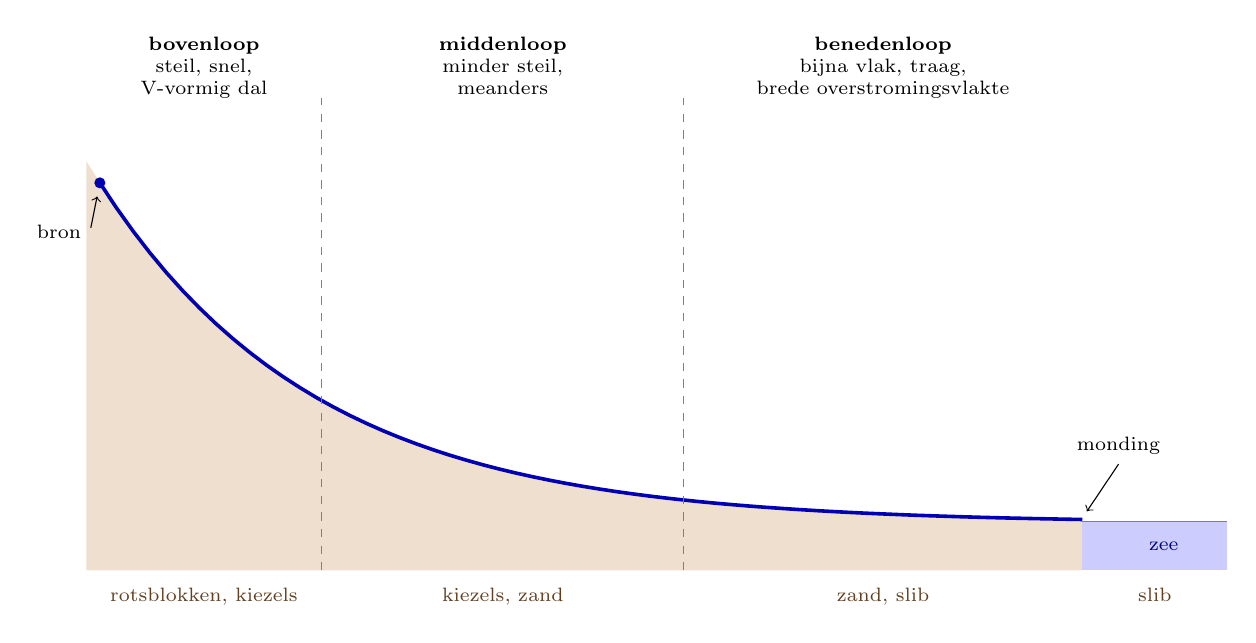
\begin{tikzpicture}[x=1.15cm, y=1cm, font=\scriptsize]
  % ground
  \fill[brown!25] (0,-0.6) -- plot[domain=0:11, samples=60]
    (\x,{4.6*exp(-\x/2.4)}) -- (11,-0.6) -- cycle;
  % sea
  \fill[blue!20] (11,-0.6) rectangle (12.6,0.02);
  \draw[blue!70!black, line width=1.3pt] plot[domain=0.15:11, samples=60]
    (\x,{4.6*exp(-\x/2.4)});
  \draw[gray] (11,0.02) -- (12.6,0.02);
  \node[blue!50!black] at (11.9,-0.3) {zee};
  % course limits
  \foreach \x in {2.6,6.6} \draw[gray, dashed] (\x,-0.6) -- (\x,5.4);
  \node[align=center, anchor=north] at (1.3,6.3) {\textbf{bovenloop}\\steil, snel,\\V-vormig dal};
  \node[align=center, anchor=north] at (4.6,6.3) {\textbf{middenloop}\\minder steil,\\meanders};
  \node[align=center, anchor=north] at (8.8,6.3) {\textbf{benedenloop}\\bijna vlak, traag,\\brede overstromingsvlakte};
  % source and mouth
  \fill[blue!70!black] (0.15,{4.6*exp(-0.15/2.4)}) circle (2pt);
  \node[anchor=east] at (0.05,3.7) {bron};
  \draw[->] (0.05,3.75) -- (0.12,4.15);
  \node[anchor=south] at (11.4,0.75) {monding};
  \draw[->] (11.4,0.75) -- (11.05,0.15);
  % grain sizes
  \node[anchor=north, align=center, text=brown!50!black] at (1.3,-0.7) {rotsblokken, kiezels};
  \node[anchor=north, align=center, text=brown!50!black] at (4.6,-0.7) {kiezels, zand};
  \node[anchor=north, align=center, text=brown!50!black] at (8.8,-0.7) {zand, slib};
  \node[anchor=north, align=center, text=brown!50!black] at (11.8,-0.7) {slib};
\end{tikzpicture}

{\small Het lengteprofiel van een \omterm{def:g1:landscapes-around-us:water}{rivier}, van \omterm{def:g5:water-shapes-the-land:source-mouth}{bron} tot \omterm{def:g5:water-shapes-the-land:source-mouth}{monding} (de hoogten
zijn sterk uitgerekt). Onder: wat er op de bodem ligt.}
\end{omfigure}

In haar \emph{bovenloop}, in de \omterm{def:g1:landscapes-around-us:landform}{bergen}, is de \omterm{def:g1:landscapes-around-us:water}{rivier} jong en steil. Haar
water raast naar beneden, rolt rotsblokken over de bodem en snijdt naar
beneden in het \omterm{def:g3:stones-pebbles-sand:rock}{gesteente}. Ze graaft een smal \omterm{def:g1:landscapes-around-us:landform}{dal} met steile wanden, in de
vorm van de letter V.

In haar \emph{middenloop} is de helling minder steil. De \omterm{def:g1:landscapes-around-us:water}{rivier} zwaait in
grote lussen van links naar rechts.

\begin{definition}[Meander]\label{def:g5:water-shapes-the-land:meander}
Een \emph{meander}\index{meander} is een lus van een \omterm{def:g1:landscapes-around-us:water}{rivier} die over een
vlakke dalbodem kronkelt.
\end{definition}

Een \omterm{def:g5:water-shapes-the-land:meander}{meander} blijft niet stil liggen: hij beweegt. Aan de buitenkant van
elke bocht stroomt het water snel en diep: het knaagt aan de oever, die een
klein steil wandje wordt. Aan de binnenkant van de bocht stroomt het water
langzaam: het laat \omterm{def:g3:stones-pebbles-sand:sand}{zand} en \omterm{def:g3:stones-pebbles-sand:pebble}{grind} vallen, die een zacht hellend strandje
opbouwen. Jaar na jaar wordt de buitenoever verder weggeslepen en groeit
het strandje in de binnenbocht, en de lus zwaait steeds wijder uit.

\begin{omfigure}
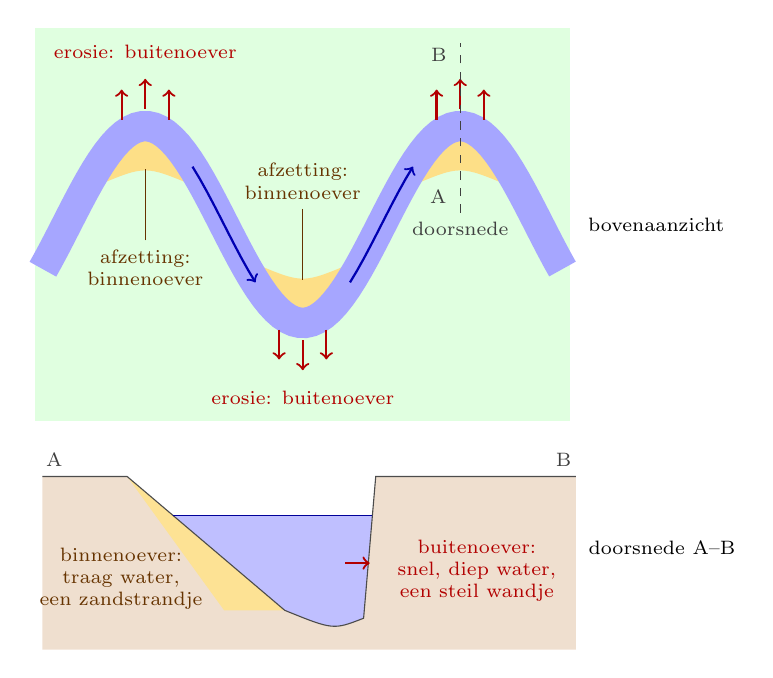
\begin{tikzpicture}[x=1cm, y=1cm, font=\scriptsize]
  % ---- map view ----
  \fill[green!12] (-0.4,-2.5) rectangle (6.4,2.5);
  % sand on the inner banks (drawn first, the river covers its edge)
  \foreach \c/\s in {1/1, 3/-1, 5/1}
    \fill[yellow!50!orange!45] (\c-0.6,\s*0.5) .. controls (\c,\s*1.5) ..
      (\c+0.6,\s*0.5) .. controls (\c,\s*0.75) .. cycle;
  % the river
  \draw[blue!35, line width=11pt] plot[domain=-0.3:6.3, samples=90]
    (\x,{1.25*sin(\x*90)});
  \draw[blue!70!black, ->, thick] plot[domain=1.6:2.4, samples=10]
    (\x,{1.25*sin(\x*90)});
  \draw[blue!70!black, ->, thick] plot[domain=3.6:4.4, samples=10]
    (\x,{1.25*sin(\x*90)});
  % erosion on the outer banks
  \foreach \c/\s in {1/1, 3/-1, 5/1}
    \foreach \d in {-0.3,0,0.3}
      \draw[red!70!black, thick, ->] (\c+\d,{\s*(1.25*cos(\d*90)+0.22)})
        -- (\c+\d,{\s*(1.25*cos(\d*90)+0.6)});
  \node[red!70!black] at (1,2.2) {erosie: buitenoever};
  \node[red!70!black] at (3,-2.2) {erosie: buitenoever};
  \node[orange!40!black, align=center] (d1) at (1,-0.55) {afzetting:\\binnenoever};
  \node[orange!40!black, align=center] (d2) at (3,0.55) {afzetting:\\binnenoever};
  \draw[orange!40!black] (d1.north) -- (1,0.7);
  \draw[orange!40!black] (d2.south) -- (3,-0.7);
  \draw[gray!50!black, dashed] (5,0.15) -- (5,2.3);
  \node[gray!50!black, anchor=north] at (5,0.15) {doorsnede};
  \node[gray!50!black, anchor=east] at (4.95,0.35) {A};
  \node[gray!50!black, anchor=east] at (4.95,2.15) {B};
  \node[anchor=west] at (6.5,0) {bovenaanzicht};
  % ---- cut ----
  \begin{scope}[yshift=-4.1cm, xscale=0.77]
    \fill[brown!25] (-0.4,-1.3) -- (-0.4,0.9) -- (1,0.9) -- (3.6,-0.8)
      .. controls (4.4,-1.05) .. (4.9,-0.9) -- (5.1,0.9) -- (8.4,0.9)
      -- (8.4,-1.3) -- cycle;
    \fill[blue!25] (1.75,0.4) -- (3.6,-0.8) .. controls (4.4,-1.05) .. (4.9,-0.9)
      -- (5.04,0.4) -- cycle;
    \fill[yellow!50!orange!40] (1,0.9) -- (3.6,-0.8) -- (2.6,-0.8) -- cycle;
    \draw[gray!60!black] (-0.4,0.9) -- (1,0.9) -- (3.6,-0.8)
      .. controls (4.4,-1.05) .. (4.9,-0.9) -- (5.1,0.9) -- (8.4,0.9);
    \draw[blue!60!black] (1.75,0.4) -- (5.04,0.4);
    \node[orange!40!black, align=center] at (0.9,-0.4) {binnenoever:\\traag water,\\een zandstrandje};
    \node[red!70!black, align=center, anchor=west] at (5.3,-0.3) {buitenoever:\\snel, diep water,\\een steil wandje};
    \draw[red!70!black, thick, ->] (4.6,-0.2) -- (5.0,-0.2);
    \node[gray!50!black, anchor=south] at (-0.2,0.9) {A};
    \node[gray!50!black, anchor=south] at (8.2,0.9) {B};
    \node[anchor=west] at (8.45,0) {doorsnede A--B};
  \end{scope}
\end{tikzpicture}

{\small Een \omterm{def:g5:water-shapes-the-land:meander}{meander} van bovenaf gezien, en in doorsnede langs de
stippellijn A--B. Het water slijt de buitenoever van elke bocht weg en legt
\omterm{def:g3:stones-pebbles-sand:sand}{zand} neer op de binnenoever: de lus verschuift langzaam.}
\end{omfigure}

Soms groeien twee lussen zo dicht naar elkaar toe dat de \omterm{def:g1:landscapes-around-us:water}{rivier} tijdens een
\omterm{def:g5:water-shapes-the-land:flood}{overstroming} door de smalle landtong ertussen breekt en de korte weg
neemt. De oude lus blijft achter als een gebogen meer.

\begin{omfigure}
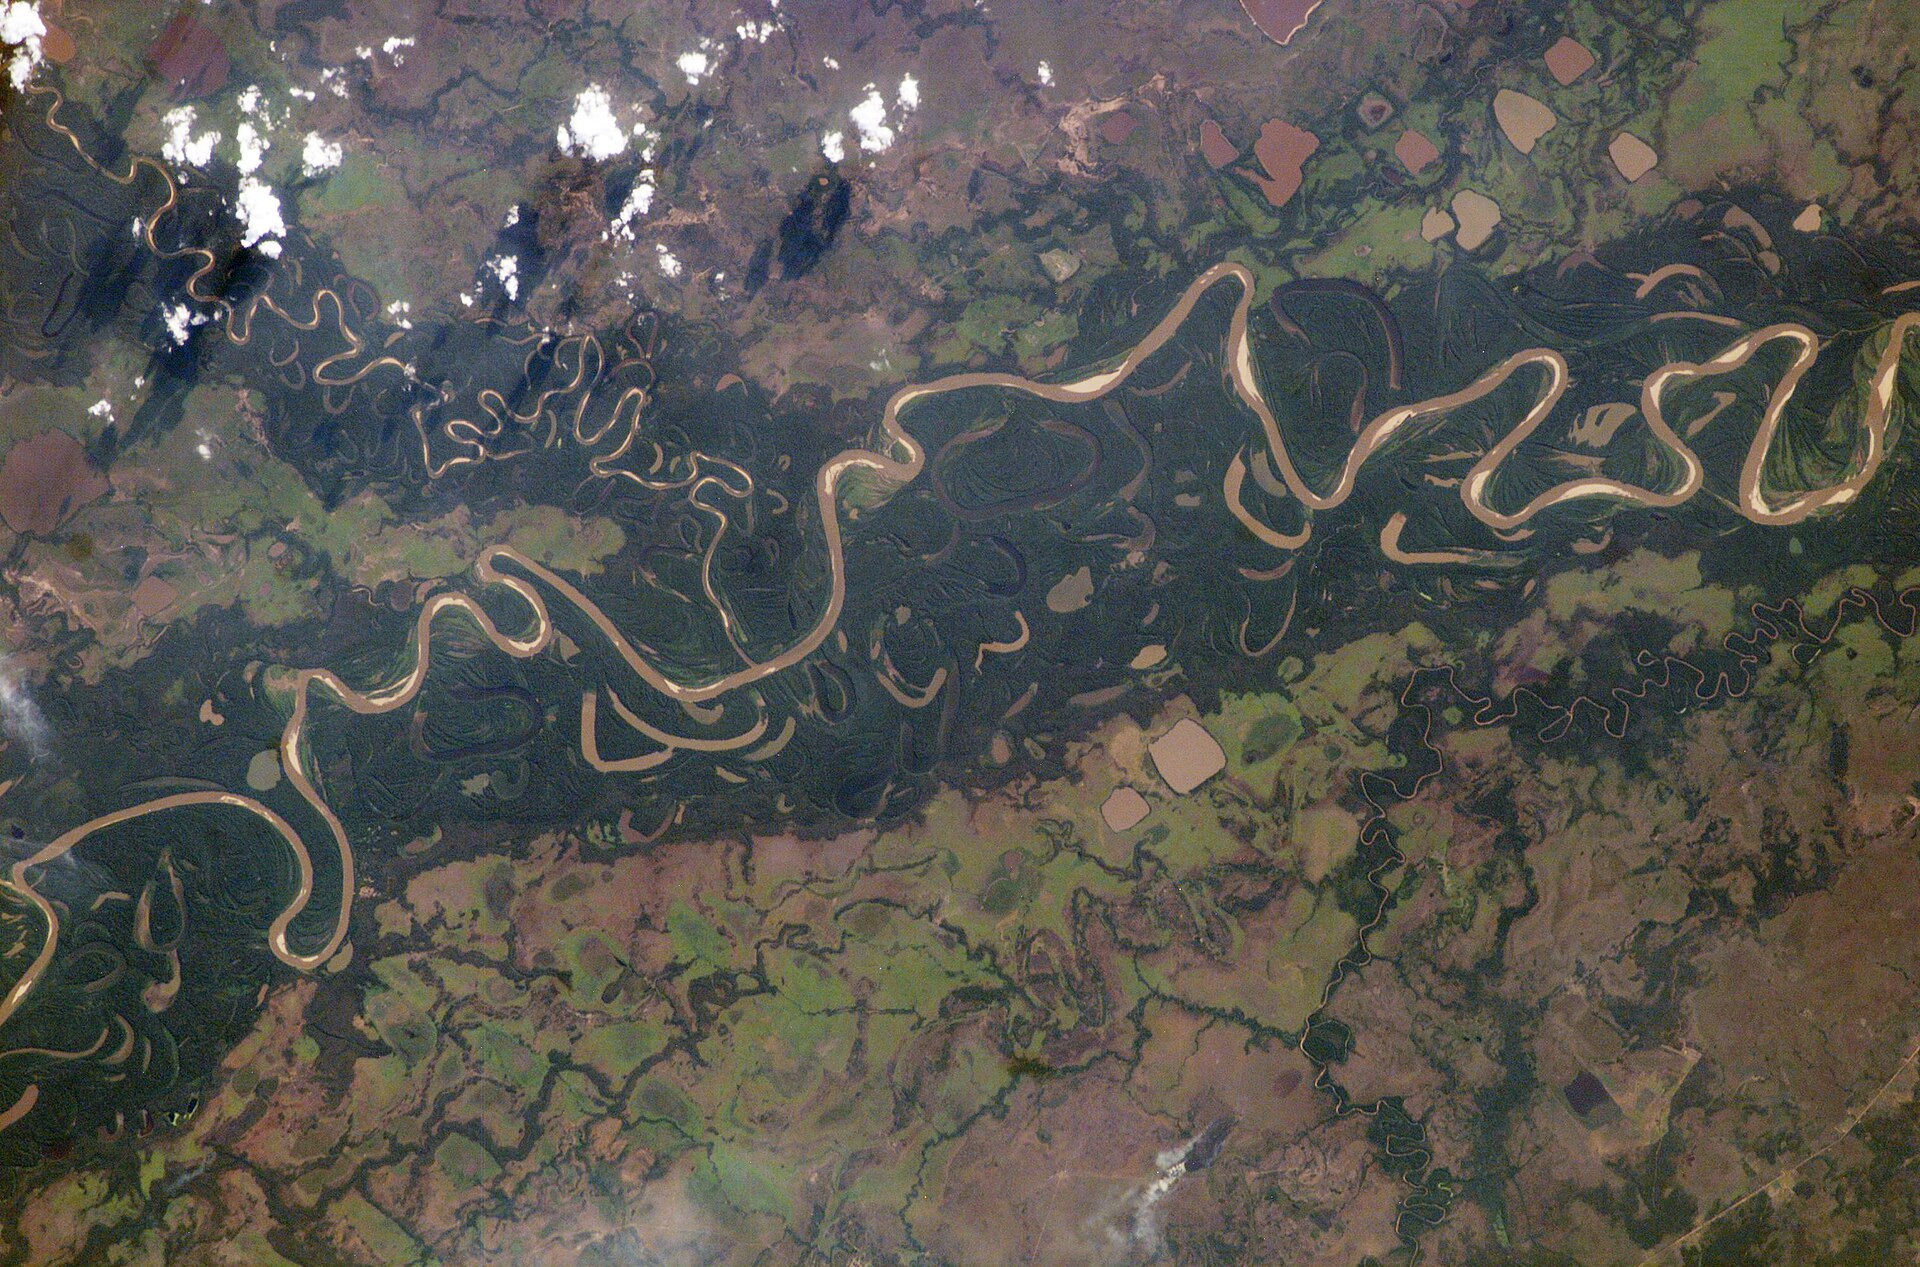
\includegraphics[width=0.52\linewidth]{images/book1/g5-mamore-meanders.jpg}

{\small De \omterm{def:g1:landscapes-around-us:water}{rivier} de Mamoré, in het laagland van Bolivia in Zuid-Amerika,
gezien vanuit het Internationaal Ruimtestation. De bruine \omterm{def:g1:landscapes-around-us:water}{rivier} kronkelt
in \omterm{def:g5:water-shapes-the-land:meander}{meanders} door het bos. Foto: NASA (publiek domein).}\label{fig:g5:water-shapes-the-land:mamore}
% ledger: nasa:mamore-meanders
\end{omfigure}

In haar \emph{benedenloop} is het land bijna vlak. De \omterm{def:g1:landscapes-around-us:water}{rivier} stroomt
langzaam over een brede, vlakke dalbodem, opgebouwd uit het \omterm{def:g3:stones-pebbles-sand:sand}{slib} en het
\omterm{def:g3:stones-pebbles-sand:sand}{zand} dat ze er zelf in heel lange tijd heeft neergelegd.

\begin{omfigure}
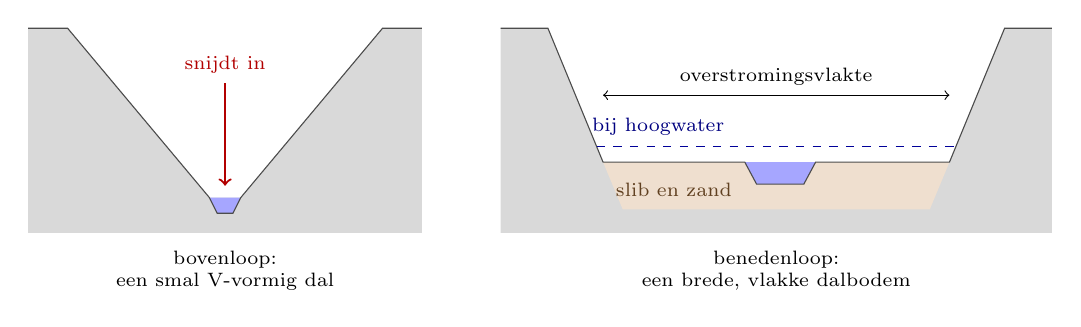
\begin{tikzpicture}[x=1cm, y=1cm, font=\scriptsize]
  % V-shaped valley
  \fill[gray!30] (0,0) -- (0,2.6) -- (0.5,2.6) -- (2.3,0.45) -- (2.7,0.45)
    -- (4.5,2.6) -- (5,2.6) -- (5,0) -- cycle;
  \fill[blue!35] (2.3,0.45) -- (2.4,0.25) -- (2.6,0.25) -- (2.7,0.45) -- cycle;
  \draw[gray!60!black] (0,2.6) -- (0.5,2.6) -- (2.3,0.45) -- (2.4,0.25)
    -- (2.6,0.25) -- (2.7,0.45) -- (4.5,2.6) -- (5,2.6);
  \draw[red!70!black, thick, ->] (2.5,1.9) -- (2.5,0.6);
  \node[red!70!black, anchor=south] at (2.5,1.9) {snijdt in};
  \node[align=center, anchor=north] at (2.5,-0.1) {bovenloop:\\een smal V-vormig dal};
  % floodplain
  \begin{scope}[xshift=6cm]
    \fill[gray!30] (0,0) -- (0,2.6) -- (0.6,2.6) -- (1.3,0.9) -- (5.7,0.9)
      -- (6.4,2.6) -- (7,2.6) -- (7,0) -- cycle;
    \fill[brown!25] (1.3,0.9) -- (1.55,0.3) -- (5.45,0.3) -- (5.7,0.9) -- cycle;
    \fill[blue!35] (3.1,0.9) -- (3.25,0.62) -- (3.85,0.62) -- (4,0.9) -- cycle;
    \draw[gray!60!black] (0,2.6) -- (0.6,2.6) -- (1.3,0.9) -- (3.1,0.9)
      -- (3.25,0.62) -- (3.85,0.62) -- (4,0.9) -- (5.7,0.9) -- (6.4,2.6) -- (7,2.6);
    \draw[blue!60!black, dashed] (1.22,1.1) -- (5.78,1.1);
    \node[blue!50!black, anchor=south] at (2.0,1.12) {bij hoogwater};
    \node[brown!50!black] at (2.2,0.55) {slib en zand};
    \draw[<->] (1.3,1.75) -- (5.7,1.75);
    \node[anchor=south] at (3.5,1.75) {overstromingsvlakte};
    \node[align=center, anchor=north] at (3.5,-0.1) {benedenloop:\\een brede, vlakke dalbodem};
  \end{scope}
\end{tikzpicture}

{\small Het \omterm{def:g1:landscapes-around-us:landform}{dal} in doorsnede, in de \omterm{def:g1:landscapes-around-us:landform}{bergen} en dicht bij de \omterm{def:g2:water-on-earth:ocean}{zee} (niet op
dezelfde schaal). Bij hoogwater breidt de \omterm{def:g1:landscapes-around-us:water}{rivier} zich uit over haar hele
\omterm{def:g5:water-shapes-the-land:flood}{overstromingsvlakte}.}
\end{omfigure}

Ten slotte bereikt de \omterm{def:g1:landscapes-around-us:water}{rivier} haar \omterm{def:g5:water-shapes-the-land:source-mouth}{monding}. Daar vertraagt het water bijna
helemaal, en de \omterm{def:g1:landscapes-around-us:water}{rivier} laat het laatste deel van haar lading vallen. Waar
de golven en de getijden van de \omterm{def:g2:water-on-earth:ocean}{zee} te zwak zijn om alles weg te voeren,
stapelen \omterm{def:g3:stones-pebbles-sand:sand}{slib} en \omterm{def:g3:stones-pebbles-sand:sand}{zand} zich op en groeit er nieuw land de \omterm{def:g2:water-on-earth:ocean}{zee} in.

\begin{definition}[Delta]\label{def:g5:water-shapes-the-land:delta}
Een \emph{delta}\index{delta} is nieuw, vlak land dat een \omterm{def:g1:landscapes-around-us:water}{rivier} bij haar
\omterm{def:g5:water-shapes-the-land:source-mouth}{monding} opbouwt uit het \omterm{def:g3:stones-pebbles-sand:sand}{slib} en het \omterm{def:g3:stones-pebbles-sand:sand}{zand} dat ze neerlegt. De \omterm{def:g1:landscapes-around-us:water}{rivier} splitst
zich in verschillende takken die zich erover verspreiden, vaak in de vorm
van een waaier.
\end{definition}

De naam komt van de Griekse letter $\Delta$ (\omterm{def:g5:water-shapes-the-land:delta}{delta}), een driehoek, omdat
de \omterm{def:g5:water-shapes-the-land:delta}{delta} van de Nijl, in Egypte, die vorm heeft.

Sommige \omterm{def:g1:landscapes-around-us:water}{rivieren} eindigen zonder \omterm{def:g5:water-shapes-the-land:delta}{delta}. Waar sterke golven en getijden het
\omterm{def:g3:stones-pebbles-sand:sand}{slib} wegvegen, eindigt de \omterm{def:g1:landscapes-around-us:water}{rivier} in een brede, trechtervormige \omterm{def:g5:water-shapes-the-land:source-mouth}{monding}
waar de \omterm{def:g2:water-on-earth:ocean}{zee} met de getijden in- en uitstroomt: een \emph{estuarium}.

\begin{omfigure}
\begin{minipage}[b]{0.55\linewidth}\centering
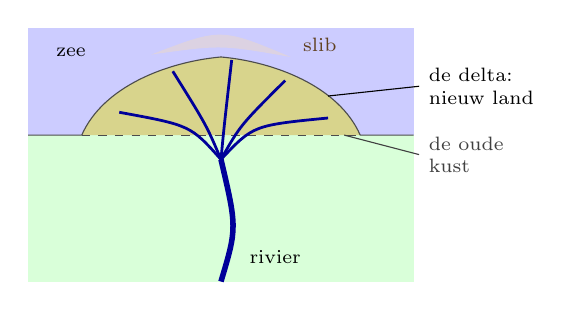
\begin{tikzpicture}[x=0.68cm, y=0.62cm, font=\scriptsize]
  \fill[blue!20] (-3.6,1.4) rectangle (3.6,3.6);
  \fill[green!15] (-3.6,-1.6) rectangle (3.6,1.4);
  % delta
  \fill[olive!35] (-2.6,1.4) .. controls (-2.2,2.4) and (-1,2.9)
    .. (0,3.0) .. controls (1,2.9) and (2.2,2.4) .. (2.6,1.4) -- cycle;
  \draw[gray!60!black] (-3.6,1.4) -- (-2.6,1.4) .. controls (-2.2,2.4) and
    (-1,2.9) .. (0,3.0) .. controls (1,2.9) and (2.2,2.4) .. (2.6,1.4) -- (3.6,1.4);
  \draw[gray!60!black, dashed] (-2.6,1.4) -- (2.6,1.4);
  % river and branches
  \draw[blue!60!black, line width=2pt] (0,-1.6) .. controls (0.3,-0.5) .. (0,0.9);
  \foreach \e in {-1.9,-0.9,0.2,1.2,2.0}
    \draw[blue!60!black, line width=1pt] (0,0.9) .. controls (\e*0.3,1.6) ..
      (\e,{2.95-0.3*\e*\e});
  % mud plume
  \fill[brown!30, opacity=0.5] (-1.3,3.05) .. controls (0,3.6) .. (1.3,3.0)
    .. controls (0,3.25) .. cycle;
  \node[align=center] at (-2.8,3.1) {zee};
  \node[anchor=west, brown!50!black] at (1.35,3.25) {slib};
  \node[anchor=west, align=left] at (3.7,2.4) {de delta:\\nieuw land};
  \draw (3.7,2.4) -- (2.0,2.2);
  \node[anchor=west, align=left, gray!50!black] at (3.7,1.0) {de oude\\kust};
  \draw[gray!50!black] (3.7,1.0) -- (2.3,1.4);
  \node[anchor=west] at (0.35,-1.1) {rivier};
\end{tikzpicture}
\end{minipage}\hfill
\begin{minipage}[b]{0.3\linewidth}\centering
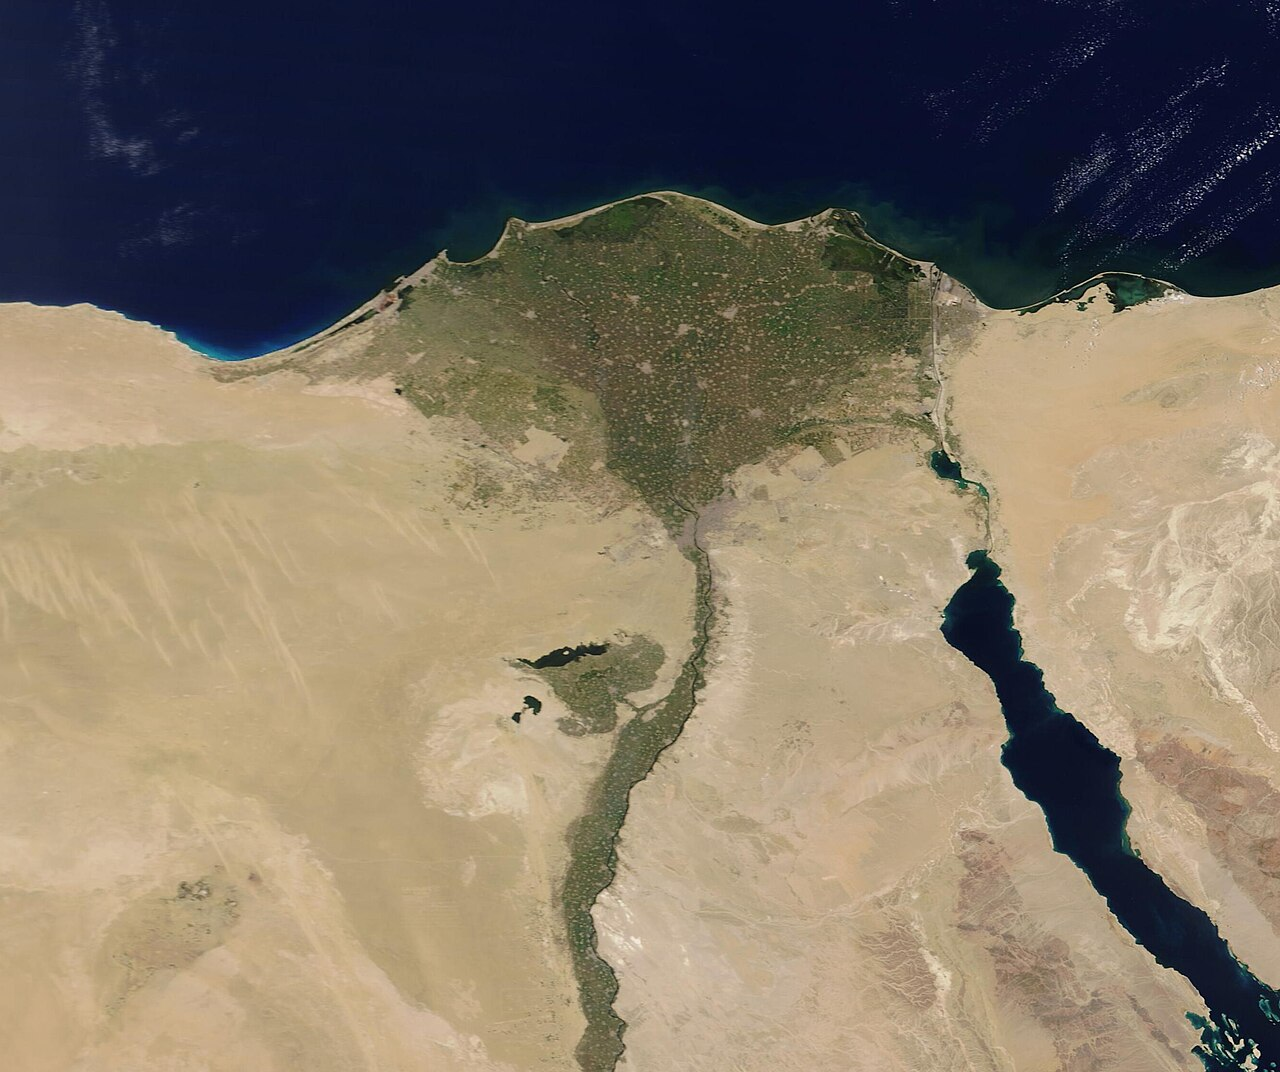
\includegraphics[width=\linewidth]{images/book1/g5-nile-delta-modis.jpg}
\end{minipage}

{\small Links: een \omterm{def:g5:water-shapes-the-land:delta}{delta} van bovenaf gezien; het \omterm{def:g3:stones-pebbles-sand:sand}{slib} en het \omterm{def:g3:stones-pebbles-sand:sand}{zand} die de
takken neerleggen, bouwen nieuw land voorbij de oude \omterm{def:g1:landscapes-around-us:water}{kust}. Rechts: de
Nijldelta, in Egypte, vanuit een satelliet (de \omterm{def:g2:water-on-earth:ocean}{zee} boven): een groene waaier
van akkers op het \omterm{def:g3:stones-pebbles-sand:sand}{slib} van de \omterm{def:g1:landscapes-around-us:water}{rivier}, midden in de woestijn. Foto: NASA
(publiek domein).}
% ledger: nasa:nile-delta-modis
\end{omfigure}

\section{Overstromingen}

Na lange dagen \omterm{def:g4:clouds-rain-snow:precipitation}{regen}, of als de \omterm{def:g4:clouds-rain-snow:precipitation}{sneeuw} in de lente snel smelt, krijgt een
\omterm{def:g1:landscapes-around-us:water}{rivier} meer water dan haar bedding kan bevatten.

\begin{definition}[Overstroming en overstromingsvlakte]\label{def:g5:water-shapes-the-land:flood}
Er is een \emph{overstroming}\index{overstroming} als water land bedekt
dat normaal droog is. Een \omterm{def:g1:landscapes-around-us:water}{rivier} treedt buiten haar oevers als ze boven
haar oevers uitstijgt en zich uitbreidt over het vlakke land aan
weerszijden. Dat vlakke land, dat de \omterm{def:g1:landscapes-around-us:water}{rivier} van tijd tot tijd bedekt, is
haar \emph{overstromingsvlakte}\index{overstromingsvlakte}.
\end{definition}

\begin{omfigure}
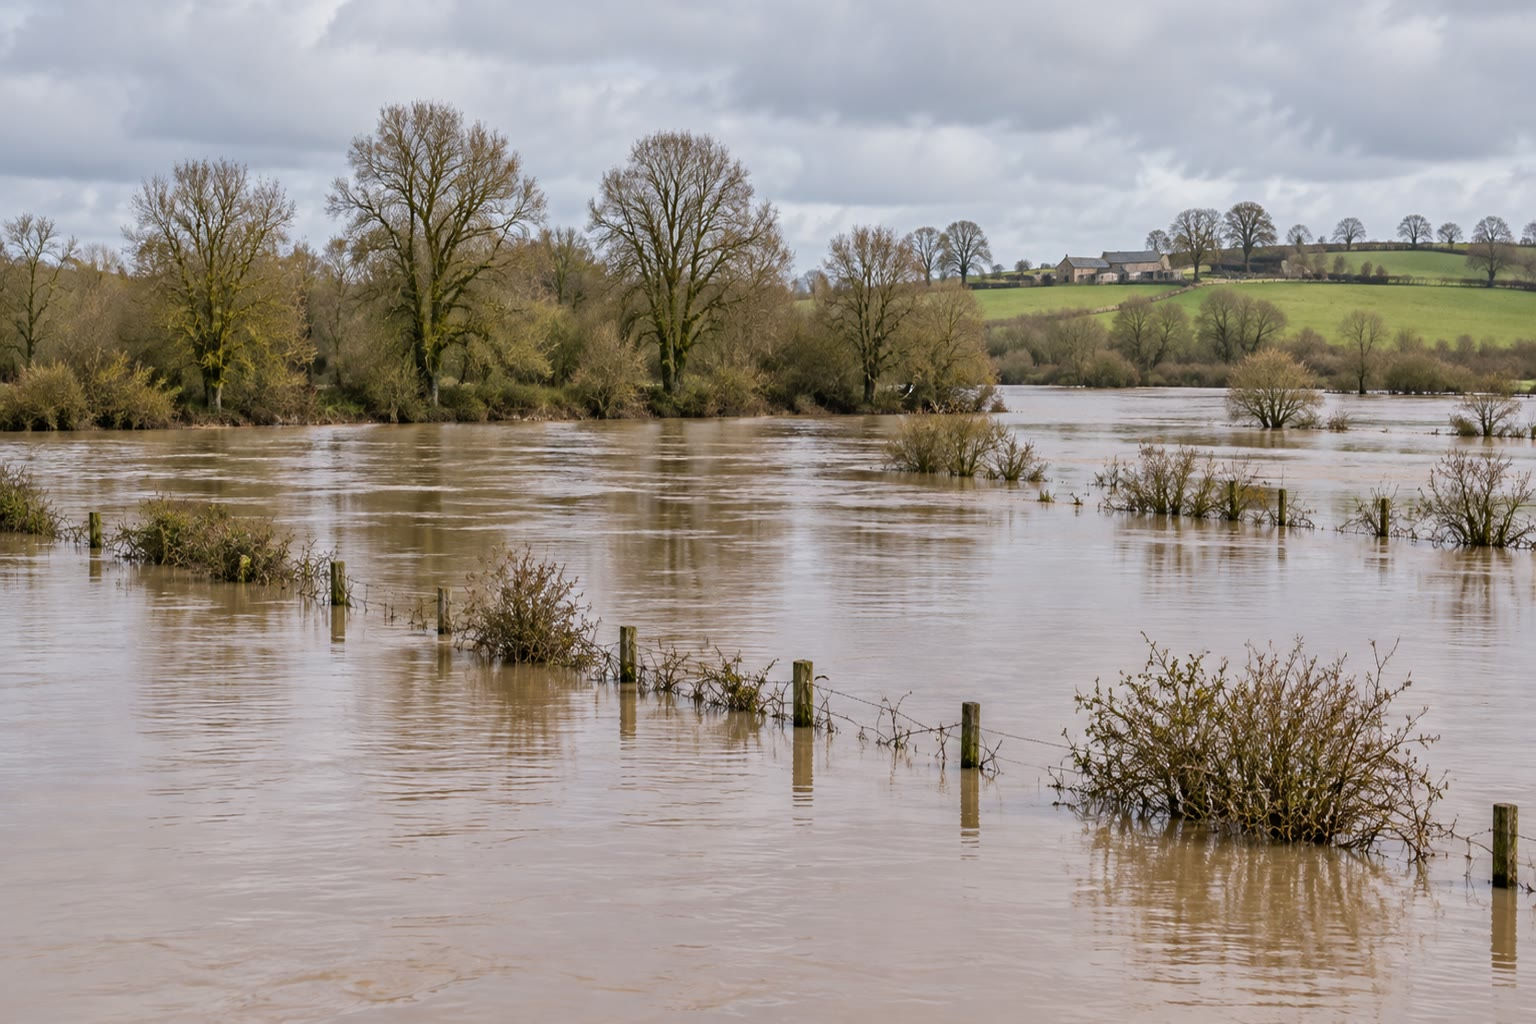
\includegraphics[width=0.5\linewidth]{images/book1/ai/g5-flooded-meadow.jpg}

{\small Een weiland onder water na dagen \omterm{def:g4:clouds-rain-snow:precipitation}{regen}. De rij bomen geeft de
gewone oever van de \omterm{def:g1:landscapes-around-us:water}{rivier} aan; de boerderij staat op hoger gelegen grond.}
\end{omfigure}

Een \omterm{def:g1:landscapes-around-us:water}{rivier} die buiten haar oevers treedt, doet niets vreemds: ze doet wat
\omterm{def:g1:landscapes-around-us:water}{rivieren} altijd hebben gedaan. De \omterm{def:g5:water-shapes-the-land:flood}{overstromingsvlakte} is haar gebied. Sterker
nog, de \omterm{def:g1:landscapes-around-us:water}{rivier} heeft die zelf gebouwd: elke \omterm{def:g5:water-shapes-the-land:flood}{overstroming} laat een dun
laagje \omterm{def:g3:stones-pebbles-sand:sand}{slib} achter op de akkers, en daarom hebben \omterm{def:g5:water-shapes-the-land:flood}{overstromingsvlakten} zo'n
vruchtbare grond. Lang geleden wachtten de boeren in Egypte op de jaarlijkse
\omterm{def:g5:water-shapes-the-land:flood}{overstroming} van de Nijl, die hun akkers bevloeide en hun nieuw \omterm{def:g3:stones-pebbles-sand:sand}{slib}
bracht.

Maar een \omterm{def:g5:water-shapes-the-land:flood}{overstroming} is gevaarlijk voor mensen die op de
\omterm{def:g5:water-shapes-the-land:flood}{overstromingsvlakte} wonen. Huizen die erop gebouwd zijn, kunnen vol water
lopen, en snel stromend water kan auto's en mensen meesleuren. Een
verstandige stad bouwt op hoger gelegen grond en laat de
\omterm{def:g5:water-shapes-the-land:flood}{overstromingsvlakte} over aan akkers, weilanden en parken. In
\cref{ch:g5:natural-hazards} zien we hoe mensen zich op \omterm{def:g5:water-shapes-the-land:flood}{overstromingen}
voorbereiden en veilig blijven.

\begin{safety}
Loop, fiets of speel nooit in overstromingswater, en ga nooit naar een
\omterm{def:g1:landscapes-around-us:water}{rivier} die buiten haar oevers is getreden: het water is sterker en dieper
dan het lijkt, en het kan gaten en open putten verbergen. Blijf weg tot de
volwassenen die de leiding hebben zeggen dat het veilig is.
\end{safety}

\section{Oefeningen}

\begin{exercise}[$\star$]\label{exo:g5:water-shapes-the-land:1}
Benoem het proces: \omterm{def:g5:water-shapes-the-land:weathering}{verwering}, \omterm{def:g5:water-shapes-the-land:erosion}{erosie} of \omterm{def:g5:water-shapes-the-land:deposition}{afzetting}?
\begin{enumerate}
  \item[(a)] IJs in een spleet splijt een rots op een \omterm{def:g1:landscapes-around-us:landform}{berg}.
  \item[(b)] Een \omterm{def:g1:landscapes-around-us:water}{rivier} die buiten haar oevers treedt, voert \omterm{def:g3:stones-pebbles-sand:sand}{zand} weg van
        haar oevers.
  \item[(c)] Een laagje \omterm{def:g3:stones-pebbles-sand:sand}{slib} zakt naar de bodem van een rustig meer.
  \item[(d)] Een boomwortel splijt een stenen muur.
\end{enumerate}
\end{exercise}

\begin{exercise}[$\star$]\label{exo:g5:water-shapes-the-land:2}
Wat is de bron van een \omterm{def:g1:landscapes-around-us:water}{rivier}? Wat is haar \omterm{def:g5:water-shapes-the-land:source-mouth}{monding}? Wat is een \omterm{def:g5:water-shapes-the-land:source-mouth}{zijrivier}?
\end{exercise}

\begin{exercise}[$\star$]\label{exo:g5:water-shapes-the-land:3}
Zet deze delen van een \omterm{def:g1:landscapes-around-us:water}{rivier} op volgorde, van de \omterm{def:g5:water-shapes-the-land:source-mouth}{bron} naar de \omterm{def:g2:water-on-earth:ocean}{zee}: de
\omterm{def:g5:water-shapes-the-land:meander}{meanders}; de \omterm{def:g5:water-shapes-the-land:delta}{delta}; het smalle V-vormige \omterm{def:g1:landscapes-around-us:landform}{dal}; de \omterm{def:g5:water-shapes-the-land:source-mouth}{bron}.
\end{exercise}

\begin{exercise}[$\star$]\label{exo:g5:water-shapes-the-land:4}
Waar of niet waar? Leg uit.
\begin{enumerate}
  \item[(a)] Hard \omterm{def:g3:stones-pebbles-sand:rock}{gesteente} verandert nooit.
  \item[(b)] Een snelle \omterm{def:g1:landscapes-around-us:water}{rivier} kan grotere stenen meevoeren dan een
        langzame \omterm{def:g1:landscapes-around-us:water}{rivier}.
  \item[(c)] Het fijnste \omterm{def:g3:stones-pebbles-sand:sand}{slib} zakt het eerst, dicht bij de \omterm{def:g5:water-shapes-the-land:source-mouth}{bron}.
\end{enumerate}
\end{exercise}

\begin{exercise}[$\star$]\label{exo:g5:water-shapes-the-land:5}
Hier zie je een bocht van een \omterm{def:g1:landscapes-around-us:water}{rivier} van bovenaf.

\begin{center}
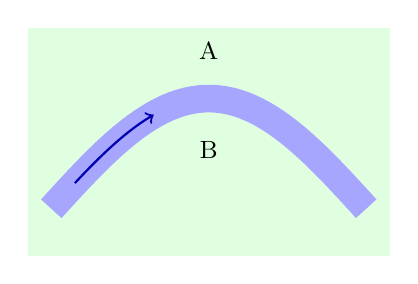
\begin{tikzpicture}[x=1cm, y=1cm, font=\small]
  \fill[green!12] (-0.3,-0.6) rectangle (4.3,2.3);
  \draw[blue!35, line width=10pt] plot[domain=0:4, samples=50]
    (\x,{1.4*sin(\x*45)});
  \draw[blue!70!black, ->, thick] plot[domain=0.3:1.3, samples=20]
    (\x,{1.4*sin(\x*45)});
  \node at (2,2.0) {A};
  \node at (2,0.75) {B};
\end{tikzpicture}
\end{center}
Op welke oever, A of B, slijt de \omterm{def:g1:landscapes-around-us:water}{rivier} het land weg? Op welke oever legt
ze \omterm{def:g3:stones-pebbles-sand:sand}{zand} neer?
\end{exercise}

\begin{exercise}[$\star$]\label{exo:g5:water-shapes-the-land:6}
In de \omterm{def:g1:landscapes-around-us:landform}{bergen} is de bodem van een \omterm{def:g1:landscapes-around-us:water}{rivier} bedekt met grote stenen. Dicht bij
de \omterm{def:g2:water-on-earth:ocean}{zee} is hij bedekt met \omterm{def:g3:stones-pebbles-sand:sand}{zand} en \omterm{def:g3:stones-pebbles-sand:sand}{slib}. Waarom?
\end{exercise}

\begin{exercise}[$\star\star$]\label{exo:g5:water-shapes-the-land:7}
Een \omterm{def:g1:landscapes-around-us:water}{rivier} is 600 kilometer lang. Haar bovenloop is het eerste
$\frac{1}{6}$ van haar lengte, en haar middenloop de volgende
$\frac{1}{2}$.
\begin{enumerate}
  \item[(a)] Hoe lang is de bovenloop? En de middenloop?
  \item[(b)] Hoe lang is de benedenloop? Welk deel van de \omterm{def:g1:landscapes-around-us:water}{rivier} is dat?
\end{enumerate}
\end{exercise}

\begin{exercise}[$\star\star$]\label{exo:g5:water-shapes-the-land:8}
Kijk nog eens naar de foto van de Mamoré vanuit het ruimtestation, op
bladzijde~\pageref{fig:g5:water-shapes-the-land:mamore}. Wat zijn de
lichte plekken aan de binnenkant van de bochten? Wat zijn de donkere,
gebogen \omterm{def:g1:landscapes-around-us:water}{meren} naast de \omterm{def:g1:landscapes-around-us:water}{rivier}? Hoe zijn ze ontstaan?
\end{exercise}

\begin{exercise}[$\star\star$]\label{exo:g5:water-shapes-the-land:9}
Een stad wil een nieuwe school bouwen in de vlakke groene weilanden naast
haar \omterm{def:g1:landscapes-around-us:water}{rivier}, omdat de grond daar vlak en goedkoop is. Wat zou je tegen de
gemeenteraad zeggen? Gebruik de woorden \emph{\omterm{def:g5:water-shapes-the-land:flood}{overstroming}} en
\emph{\omterm{def:g5:water-shapes-the-land:flood}{overstromingsvlakte}}.
\end{exercise}

\begin{exercise}[$\star\star$]\label{exo:g5:water-shapes-the-land:10}
De \omterm{def:g1:landscapes-around-us:water}{rivieren} van de wereld brengen elk jaar ongeveer 12 miljard ton \omterm{def:g3:stones-pebbles-sand:sand}{slib} en
\omterm{def:g3:stones-pebbles-sand:sand}{zand} naar de \omterm{def:g2:water-on-earth:ocean}{zee}.
\begin{enumerate}
  \item[(a)] Hoeveel ton is dat gemiddeld per maand?
  \item[(b)] Een grote vrachtwagen vervoert 10 ton. Hoeveel
        vrachtwagenladingen zijn er nodig om het \omterm{def:g3:stones-pebbles-sand:sand}{slib} en \omterm{def:g3:stones-pebbles-sand:sand}{zand} van één maand
        te vervoeren?
\end{enumerate}
\end{exercise}

\begin{exercise}[$\star\star\star$]\label{exo:g5:water-shapes-the-land:11}
Vertel het verhaal van een zandkorrel. Hij begint als deel van een rots
hoog op een \omterm{def:g1:landscapes-around-us:landform}{berg}, en hij eindigt, vele jaren later, in een \omterm{def:g5:water-shapes-the-land:delta}{delta}. Gebruik
de woorden \emph{\omterm{def:g5:water-shapes-the-land:weathering}{verwering}}, \emph{\omterm{def:g5:water-shapes-the-land:erosion}{erosie}} en \emph{\omterm{def:g5:water-shapes-the-land:deposition}{afzetting}}, en vertel
wat er met de korrel gebeurt in de bovenloop, de middenloop en de
benedenloop van de \omterm{def:g1:landscapes-around-us:water}{rivier}.
\end{exercise}
